\chapter{Análisis de requisitos}
\label{chap:requisitos}
\section{Funcionalidades}
Esta aplicación dispoñerá de catro funcionalidades principais:
\begin{itemize}

    \item \textbf{Menú principal}: Funcionalidade "de enlace" co resto das funcionalidades. É a base da aplicación.
    
    \item \textbf{Dicionario}: Apoiarase nunha base de datos deseñada con \textit{Room} para gardar as palabras e poder seleccionar unha aleatoriamente á hora de comezar unha partida. Poderanse eliminar e engadir palabras. Non se permitirá utilizar o dicionario baleiro no resto de funcionalidades. Non se poderá introducir unha palabra maior a 17 caracteres por cuestión de espazo. Haberá comprobación dos caracteres introducidos.
    
    \item \textbf{Modo un xogador}: Esta funcionalidade consistirá en permitir ao usuario poder xogar de maneira individual. Neste caso, a aplicación escollerá unha palabra aleatoria dende un dicionario (podendo ser este ampliable polos usuarios) situado nos propios arquivos da aplicación e presentaralla ao usuario por pantalla para que trate de adiviñala.
    
    
    \item \textbf{Modo multixogador}: Nesta funcionalidade permitirase xogar a máis dun usuario enfrentarse entre eles. O funcionamento segue o mesmo modo que o dun xogador pero cun contador no que se amosa o tempo restante para elexir unha letra. Se este tempo expira, o xogador será eliminado. Gañará o xogador con menos erros ou o que quede sen ser eliminado, en caso de empate haberá varios gañadores. Esta funcionalidade encárgase da parte de autencicación de usuarios e comunicacións en liña.
    
\end{itemize}

A prioridade de implementación das funcionalidades seguirá a orde descrita anteriormente, sendo o menú principal a primeira funcionalidade en ser implementada, o modo multixogador o último.\\
\begin{center}
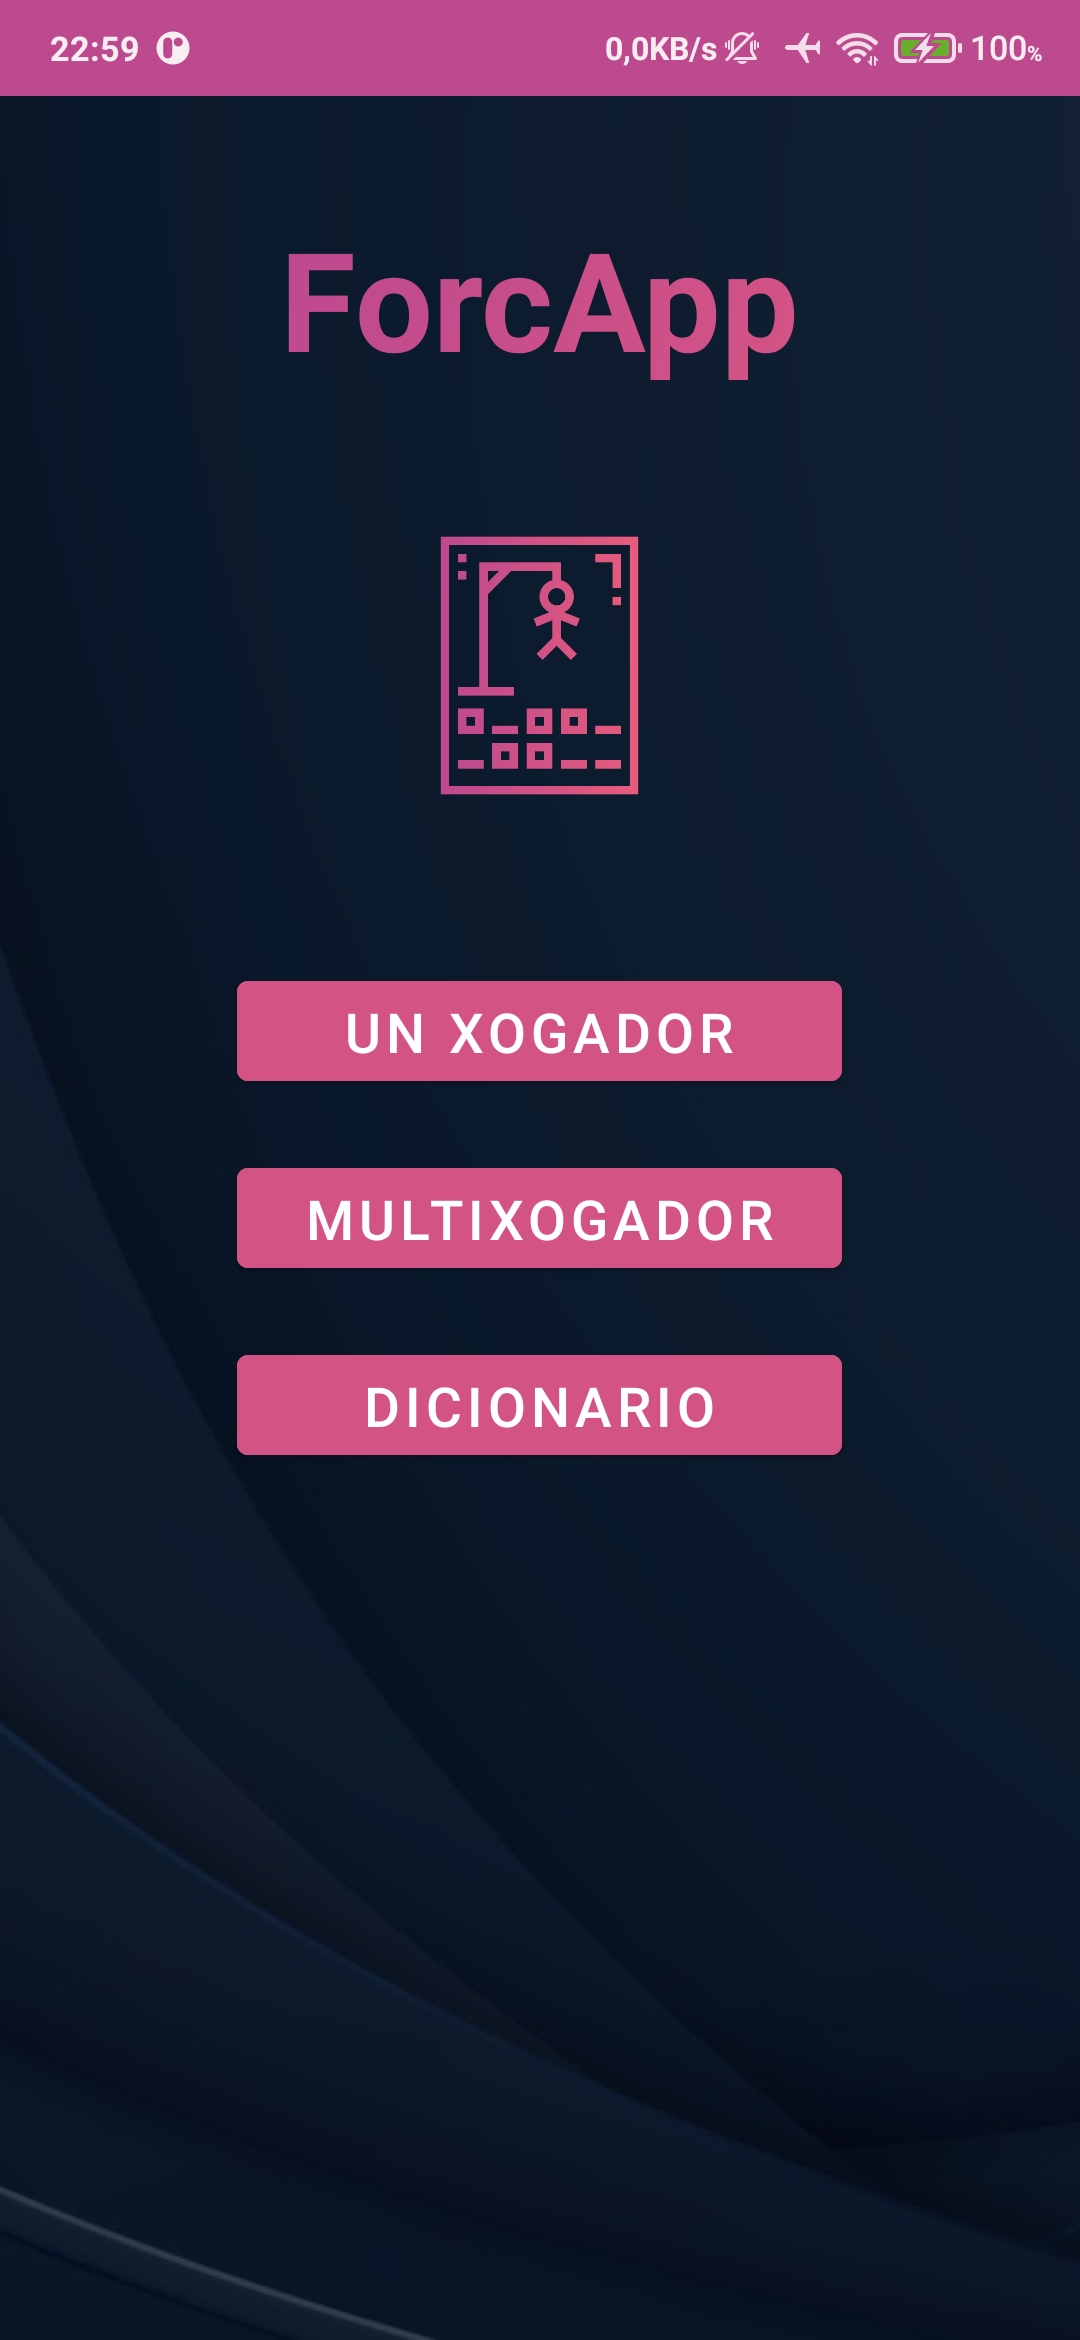
\includegraphics[scale=0.15]{imaxes/menu.jpg}
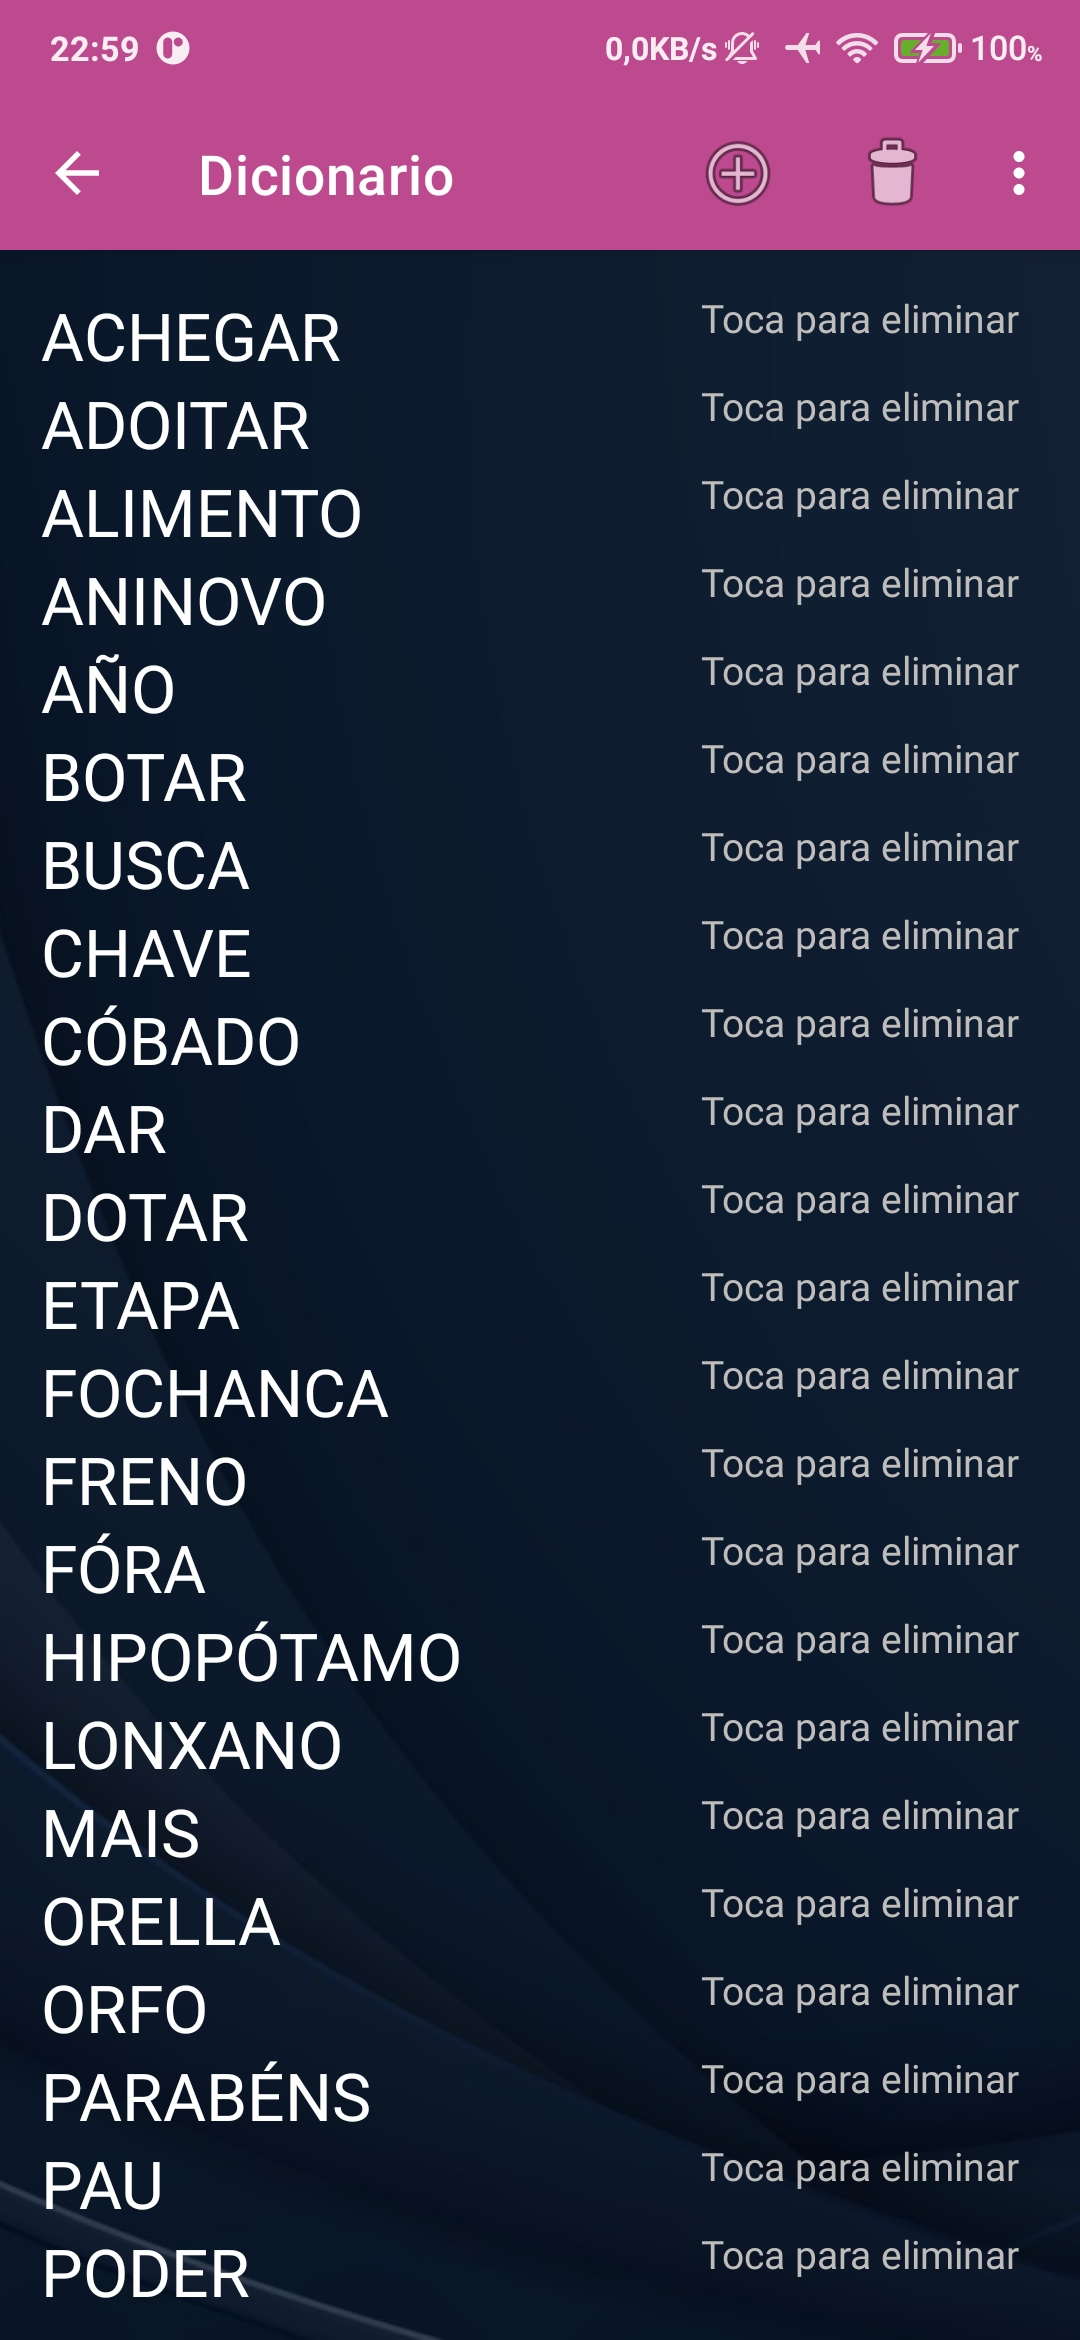
\includegraphics[scale=0.15]{imaxes/dicionario.jpg}
\end{center}
\begin{center}
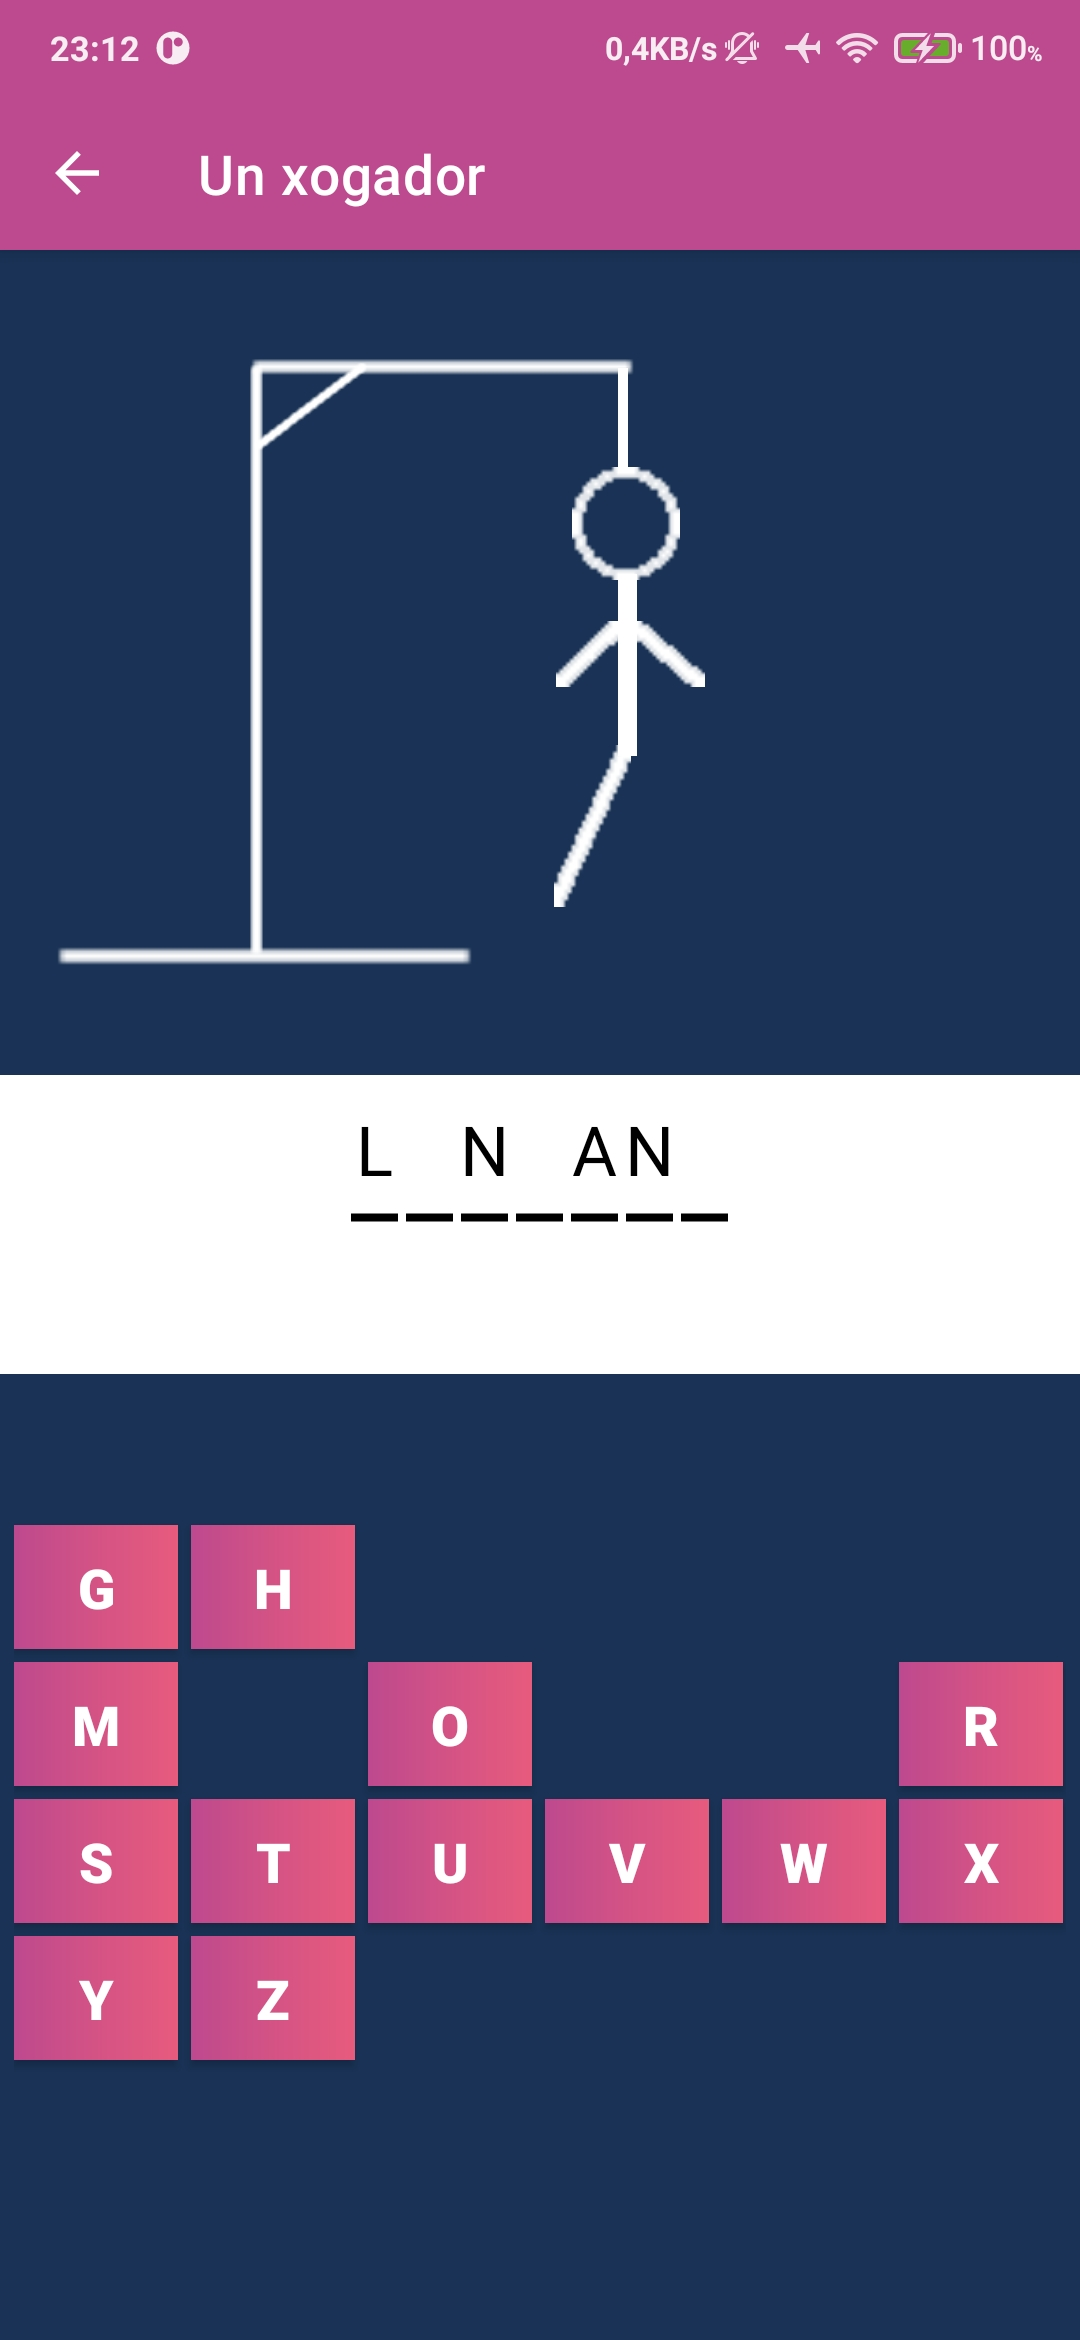
\includegraphics[scale=0.15]{imaxes/singleplayer.jpg}
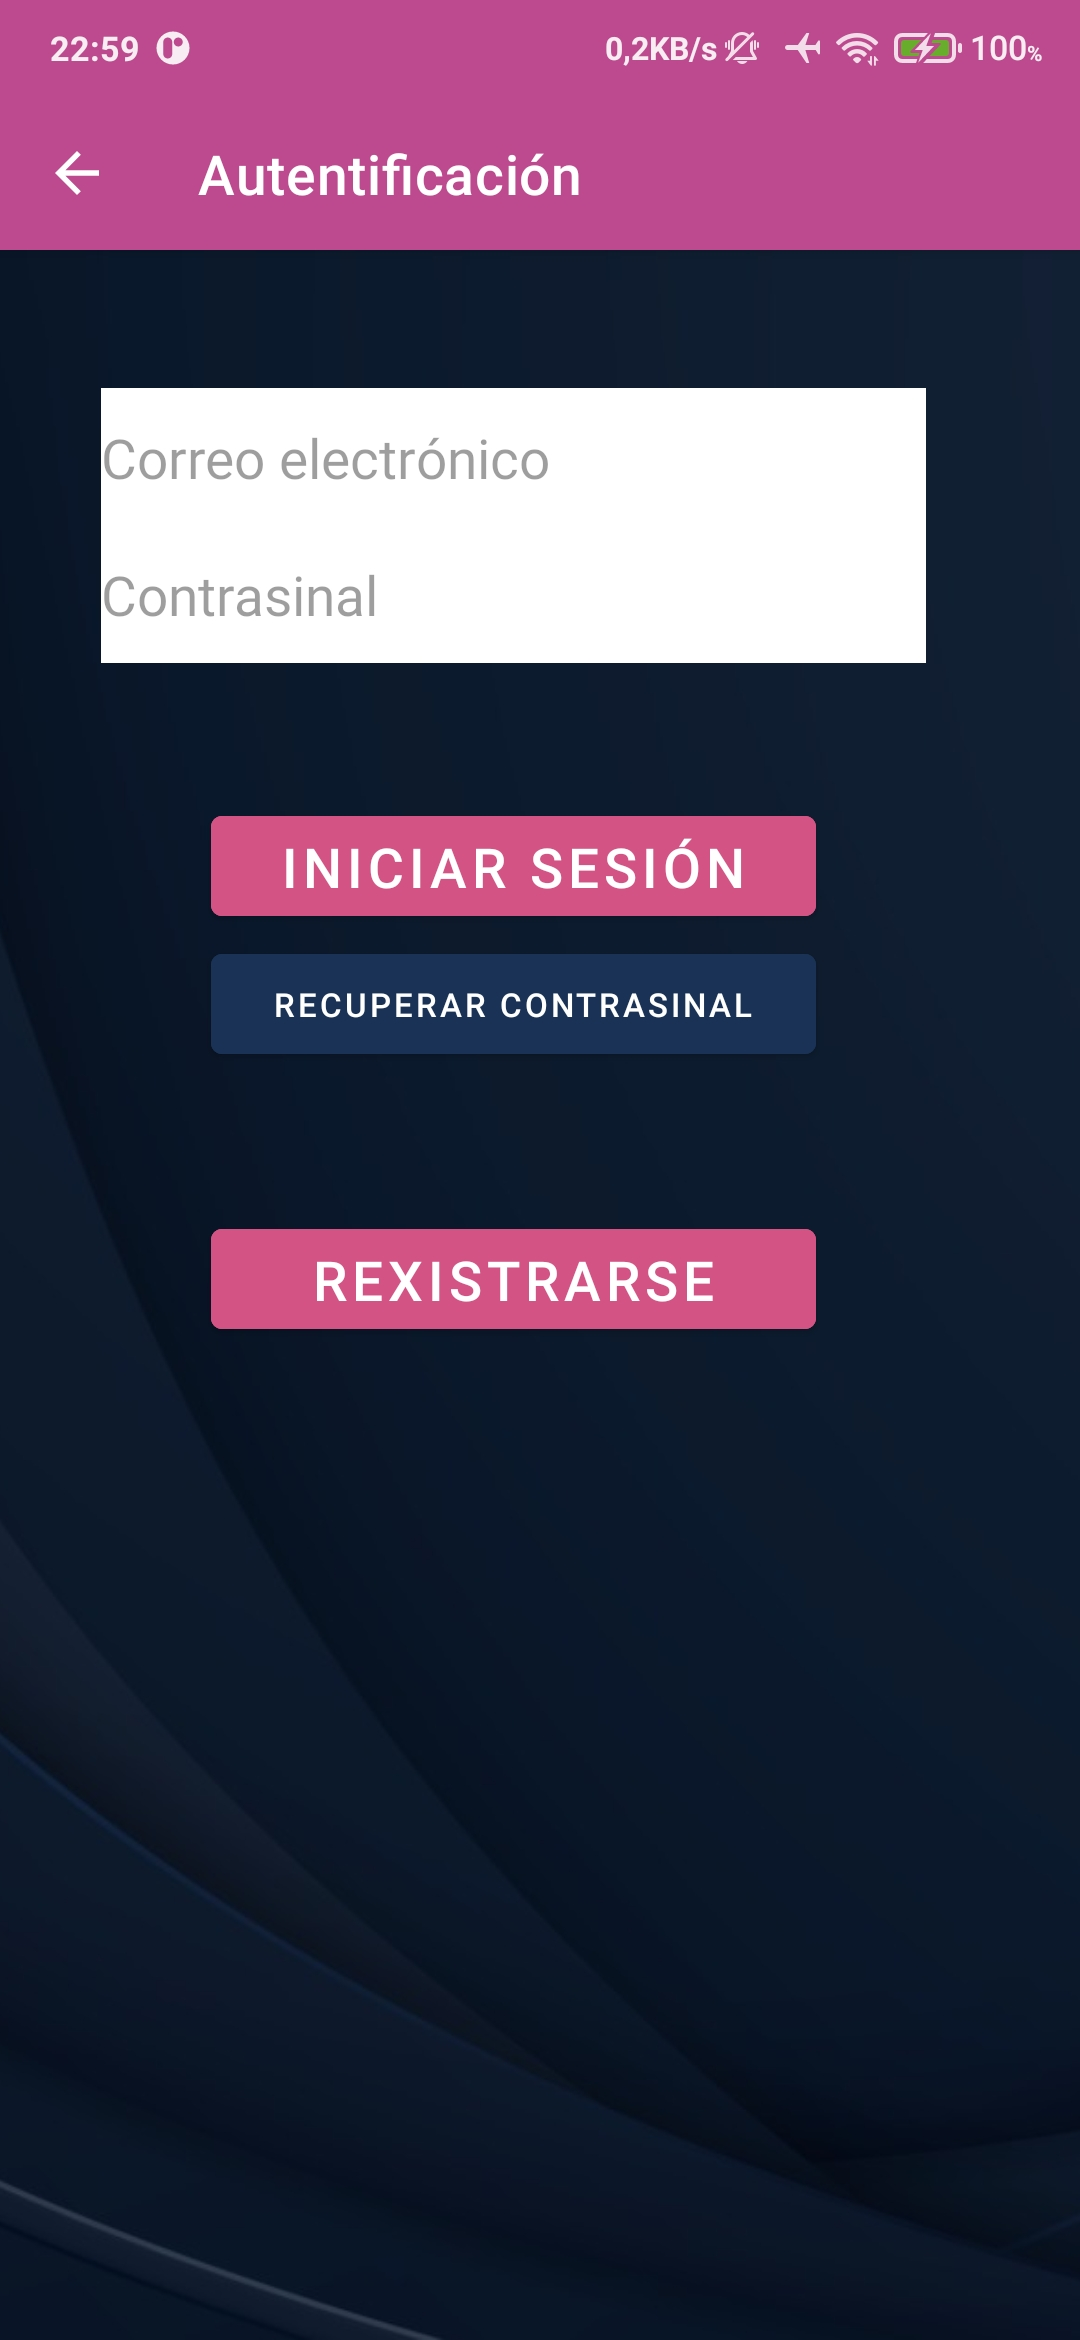
\includegraphics[scale=0.15]{imaxes/auth.jpg}\\ [30 pt]
\end{center}
En traballos futuros pódense engadir novas funcionalidades como levar a conta de partidas gañadas e perdidas (pódense calcular estatísticas como porcentaxes de éxito ou número de intentos medios para obter unha victoria) en calquera dos dous modos, para esto faría falta outra base de datos a maiores.\\

Ademais a aplicación amosará un teclado 'artificial' sen necesidade de usar un do sistema. Ao seleccionar unha letra dese teclado amosarase sombreada e non será posible volver a seleccionala.
 \let\cleardoublepage=\clearpage 